\documentclass[a4paper,10pt]{article}
\usepackage[spanish]{babel}
\usepackage[latin1]{inputenc}
\usepackage{anysize} % Soporte para el comando \marginsize
\usepackage{listings}
\usepackage{formular}
\usepackage[pdftex]{graphicx}
\usepackage{setspace}
\usepackage{booktabs}



\DeclareGraphicsExtensions{.pdf,.png,.jpg}

\usepackage{color}
\definecolor{gray97}{gray}{.97}
\definecolor{gray75}{gray}{.75}
\definecolor{gray45}{gray}{.45}

\lstset{ frame=Ltb,
     framerule=0pt,
     aboveskip=0.5cm,
     framextopmargin=3pt,
     framexbottommargin=3pt,
     framexleftmargin=0.4cm,
     framesep=0pt,
     rulesep=.4pt,
     backgroundcolor=\color{gray97},
     rulesepcolor=\color{black},
     %
     stringstyle=\ttfamily,
     showstringspaces = false,
     basicstyle=\small\ttfamily,
     commentstyle=\color{gray45},
     keywordstyle=\bfseries,
     %
     numbers=left,
     numbersep=15pt,
     numberstyle=\tiny,
     numberfirstline = false,
     breaklines=true,
   }

% minimizar fragmentado de listados
\lstnewenvironment{listing}[1][]
   {\lstset{#1}\pagebreak[0]}{\pagebreak[0]}

\lstdefinestyle{consola}
   {basicstyle=\scriptsize\bf\ttfamily,
    backgroundcolor=\color{gray75},
   }

\lstdefinestyle{C}
   {language=C,
   }


\renewcommand*\lstlistingname{Listado}


\marginsize{3cm}{3cm}{2.5cm}{2.5cm}
\setlength{\parindent}{25pt}

%opening
\title{\textbf{ Wireless communications
in NS3}\\ Simulating wireless communications}
\author{Alejandro Juli\'an Ferro Bejerano}

\begin{document}


\maketitle

\begin{figure}[!h]
\centering
   
\includegraphics[width=8cm]{escudo_esi.jpg}
\end{figure}

\newpage

\tableofcontents

\newpage

\section{Objetives}

The main objective of this documents is to understand wireless communications and guide student in
its first simulation process through NS3 simulator.

\singlespacing
To do so, we will answer some fundamental questions. Let's look

\section{Changing the script}
Starting with the original example stats and responds as would the following activities.

\subsection{increment the distances used in each iteration of the simulation to: 25 50 75 100 125 145 147
150 152 155 157 160 162 165 167 170 172 175 177 180 185 190 195 200 210 220 230 240 250
300 350 400 450 500 600 750 1000}

\singlespacing
To resolve this issue we edit the \textbf{wifi-example-db.sh} file by changing the values of the variable "Distances"

\begin{lstlisting}[style=C]
-db.sh
#!/bin/sh

DISTANCES="25 50 75 100 125 145 147 150 152 155 157 160 162 165 167 170 172 175 177 180 185 190 195 200 210 220 230 240 250 300 350 400 450 500 600 750 1000"
(...)
\end{lstlisting}

\subsection{Reduce the number of iterations for each distance from five to one}

\singlespacing
Same as above case but editing the variable "Trials"

\begin{lstlisting}[style=C]
-db.sh
#!/bin/sh

DISTANCES="25 50 75 100 125 145 147 150 152 155 157 160 162 165 167 170 172 175 177 180 185 190 195 200 210 220 230 240 250 300 350 400 450 500 600 750 1000"
TRIALS="1"

(...)
\end{lstlisting}


\subsection{Adjust the x-axis of the gnuplot script to show results of the new distance}

\singlespacing
To adjust the x-axis of the gnuplot we only need edit the \textbf{wifi-example.gnuplot} as we show and change the value of the \emph{xrange}

\begin{lstlisting}[style=C]
(...)
#--------- x-axis adjust --------------
set xrange [0:1500]
#--------------------------------------
(...)
\end{lstlisting}


\begin{figure}[h]
        	\centering
    \includegraphics[scale=0.55]{wifi-default.eps}
    \caption{Graphic generated by example stats of NS3 with previous amendments}
    \label{fig:inicio}
        \end{figure}


\section{Changing the antenna parameters of simulation}

\subsection{which object represents the antenna? Which properties do you should change for increase the range
of a successful communication?}

\singlespacing
The object representing the antenna is \textbf{wifiPhy} and we should change the profits of reception and transmission.

\subsection{To study the values of the properties to change in order to establish a successfully communication
of 400 meters}

\singlespacing
As discussed in the previous question for successful communication, we need to edit the file \textbf{wifi-example-sim.cc}. This left in the following way.

\begin{lstlisting}[style=C]
(...)
  //--------------------------------------------
  //-- Create nodes and network stacks
  //--------------------------------------------
  NS_LOG_INFO ("Creating nodes.");
  NodeContainer nodes;
  nodes.Create (2);

  NS_LOG_INFO ("Installing WiFi and Internet stack.");
  WifiHelper wifi = WifiHelper::Default ();
  NqosWifiMacHelper wifiMac = NqosWifiMacHelper::Default ();
  wifiMac.SetType ("ns3::AdhocWifiMac");
  YansWifiPhyHelper wifiPhy = YansWifiPhyHelper::Default ();
  #--- profits of transmission and reception ---
  wifiPhy.Set("RxGain",DoubleValue(10));
  wifiPhy.Set("TxGain",DoubleValue(10));
  #---------------------------------------------
  YansWifiChannelHelper wifiChannel = YansWifiChannelHelper::Default ();
  wifiPhy.SetChannel (wifiChannel.Create ());
  NetDeviceContainer nodeDevices = wifi.Install (wifiPhy, wifiMac, nodes);

(...)
\end{lstlisting}


\begin{figure}[h]
        	\centering
    \includegraphics[scale=0.55]{wifi-400.eps}
    \caption{Graphic generated by example stats of NS3 with previous amendments}
    \label{fig:inicio}
        \end{figure}


\section{The loss model}

\subsection{Surf in the NS3 help and list the different types of loss propagation models implemented}
\begin{itemize}
\item x

\item x

\item x

\end{itemize}


\begin{table}[htbp]
\centering
\begin{tabular}{p{2cm} p{10cm}}
\hline \hline
Se eliminan ``charter - '' y `` - charter''&\\
\hline
Se eliminan ``- air taxi'' y ``Air Taxi -''&\\
\hline \hline

\end{tabular}
\caption{Campo ``Operator''.}
\label{tabla:autores}
\end{table}



\singlespacing
\begin{table}[htbp]
\centering
\begin{tabular}{p{3cm} p{7cm}}
\hline \hline
Campos eliminados& Descripci\'on\\
\hline \hline
Fatalities &Total de muertes a bordo, se sustituir\'a por dos nuevos campos, Fatalities\_Passengers y Fatalities\_Crew\\
\hline
Abordo&Total de personas a bordo,ser\'a sustituido por Aboard\_Passengers y Aboard\_Crew\\
\hline
Route & Indica la ruta completa o parcial antes de producirse el accidente, incluyendo las escalas. Se sustituir\'a por los campos Origen, Destino, y Escalas\\
\hline \hline
\end{tabular}
\caption{Campos eliminados.}
\label{tabla:autores}
\end{table}
\pagebreak
\begin{table}[htbp]
\centering
\begin{tabular}{p{5cm} p{5cm}}
\hline \hline
Campos introducidos &Descripci\'on\\
\hline \hline
\hline
Fatalities\_Passengers &N\'umero total de pasajeros fallecidos\\
\hline
Fatalities\_Crew&N\'umero total de tripulaci\'on fallecida\\
\hline
Aboard\_Passengers & N\'umero total de pasajeros a bordo\\
\hline
Aboard\_Crew &N\'umero otal de tripulaci\'on a bordo\\
\hline
Origen&El primer elemento del campo ``Route''\\
\hline
Destino& El \'ultimo elemento del campo ``Route''\\
\hline
Escalas & Los elementos intermedios entre Origen y Destino del campo ``Route'' o ´´ '' si no existe ninguno\\
\hline
Latitude/Longitud\_Location & Latitud  y longitud del lugar del accidente\\
\hline
Latitude/Longitude\_Origen&Latitud  y longitud del lugar del origen del vuelo\\
\hline
Latitude/Longitude\_Destino&Latitud  y longitud del lugar del destino del vuelo\\
\hline \hline
\end{tabular}
\caption{Campos eliminados.}
\label{tabla:autores}
\end{table}



\section{Webgraf\'ia y herramientas}
\begin{itemize}
\item https://www.nsnam.org/doxygen/
\item \LaTeX
\end{itemize}



\end{document}
